\section{Рабочий проект}
\subsection{Классы, используемые при разработке сайта}

Можно выделить следующий список классов и их методов, использованных при разработке игры (таблица \ref{class:table}).

\renewcommand{\arraystretch}{0.8} % уменьшение расстояний до сетки таблицы
\begin{xltabular}{\textwidth}{|X|p{2.5cm}|>{\setlength{\baselineskip}{0.7\baselineskip}}p{4.85cm}|>{\setlength{\baselineskip}{0.7\baselineskip}}p{4.85cm}|}
\caption{Описание классов, используемых в приложении\label{class:table}}\\
\hline \centrow \setlength{\baselineskip}{0.7\baselineskip} Название класса & \centrow \setlength{\baselineskip}{0.7\baselineskip} Модуль, к которому относится класс & \centrow Описание класса & \centrow Методы \\
\hline \centrow 1 & \centrow 2 & \centrow 3 & \centrow 4\\ \hline
\endfirsthead
\caption*{Продолжение таблицы \ref{class:table}}\\
\hline \centrow 1 & \centrow 2 & \centrow 3 & \centrow 4\\ \hline
\finishhead
Animation & Модуль графики & Animation – Класс анимации игры. Создает анимации и хранит все информацию о её состоянии & def onTimetAnimation(self) Счетчик кадров анимации

def get\_frame(self) Возвращает текущий кадр

def crop(self) Разбиение на кадры

def rotateImg(self, img, t) Вращение изображения, img : PhotoImage изображение, t : str действие. Возвращает повернутое на 90 или 180 градусов изображение или отзеркаливает его

def makeTransparent(self, img) Прозрачность изображения, img : PhotoImage изображение. Возвращает изображение, удаляя весь белый цвет\\
\hline GameObject & Модуль логики & GameObject – Класс игровых объектов & def change\_anim(self, name) Изменение текущей анимации объекта, name : str ключ анимации

def find\_animation(self, name) Поиск анимации по названию, name : str название анимации. Возвращает анимация с названием\\
\hline Graphics & Модуль графики & Graphics – Класс отображения игрового движка & def change\_frame(self, id, img) Смена кадра анимации, id : int id объекта, sprite : PhotoImage кадр анимации

def add\_anim(self) Добавляет анимацию в словарь

def onTimer(self) Цикл анимаций\\
\hline Game & Модуль логики & Game – Класс игрового движка & def initGame(self) Инициализация всех начальных значений для переменных

def loadImages(self) Загрузка начальных спрайтов

def bind(self, up, left, right) Установка клавиш управления, up : str клавиша прыжка, left : str клавиша движения влево, right : str клавиша движения вправо

def movePlayer(self) Передвижение спрайта игрока

def create\_map(self, level, widht) Создание карты по массиву, level : list[str] массив с ключами, widht : int ширина клетки на карте в пикселях

def add\_gameobjects(self, tag) Добавляет к списку объектов все объекты с тегом, tag : str тег объектов

def find\_objects\_tag(self, tag) Возвращает список объектов с тегом, tag : str тег объектов

def find\_object\_id(self, id) Возвращает объект с соответствующим id, id : int id объекта\\
\hline  &  &  & def checkCollisions(self, anchor) Проверка коллизий игрока, anchor : str направление движения игрока

def checkWallCollision(self, x1, x2, y1, y2, anchor, key) Проверка коллизий со стенами, x1 : int, x2 : int, y1 : int, y2 : int
координаты, anchor : str направление движения игрока, key : str нажатая клавиша

def change\_animation(self, id, name) Изменяет текующую анимацию объекта, id : int id объекта, name : str ключ анимации

def add\_animations(self) Добавление анимаций

def onTimer(self) Игровой цикл\\
\hline MyGame & Главный модуль & Game – Класс игры & def run(self) Запуск mainloop для Tk

def update(self) Обновление игры Запускает основной цикл

def keys(self, keyup, keyleft, keyright) Установка клавиш управления, keyup : str клавиша прыжка, keyleft : str клавиша движения влево, keyright : str клавиша движения вправо

def onKeyPressed(self, e) Вызывается при нажатии клавиш на клавиатуре

def onKeyRelease(self, e) Вызывается при отжатии клавиш на клавиатуре

def drawScore(self) Отрисовка счета

def endGame(self) Выводит сообщение в конце игры

\end{xltabular}
\renewcommand{\arraystretch}{1.0} % восстановление сетки

\subsection{Системное тестирование разработанной игры}

На рисунке \ref{main:image} представлено главное окно игры.
\newpage % при необходимости можно переносить рисунок на новую страницу
\begin{figure}[H] % H - рисунок обязательно здесь, или переносится, оставляя пустоту
\center{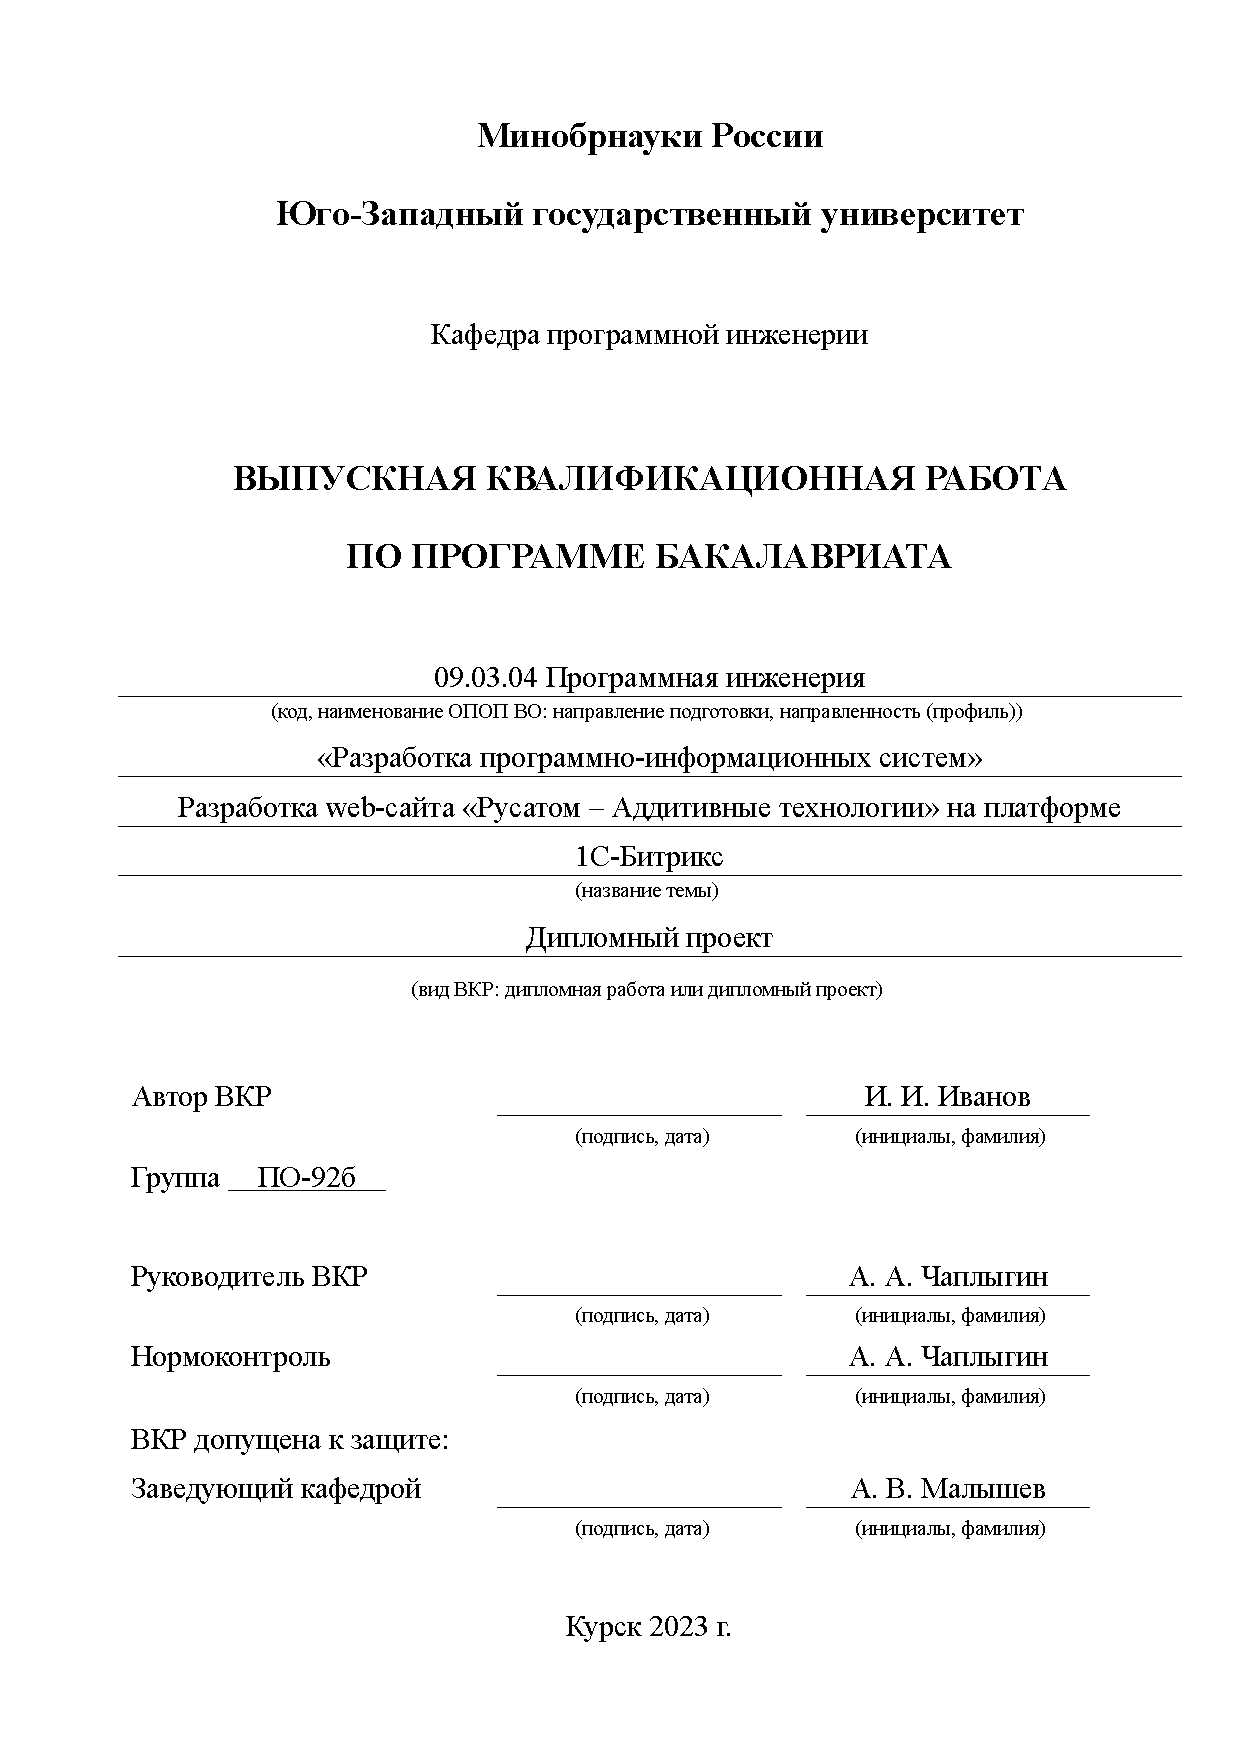
\includegraphics[width=1\linewidth]{main}}
\caption{Главное окно игры}
\label{main:image}
\end{figure}

На рисунке \ref{menu:image} игрок собрал несколько монет.

\begin{figure}[ht]
\center{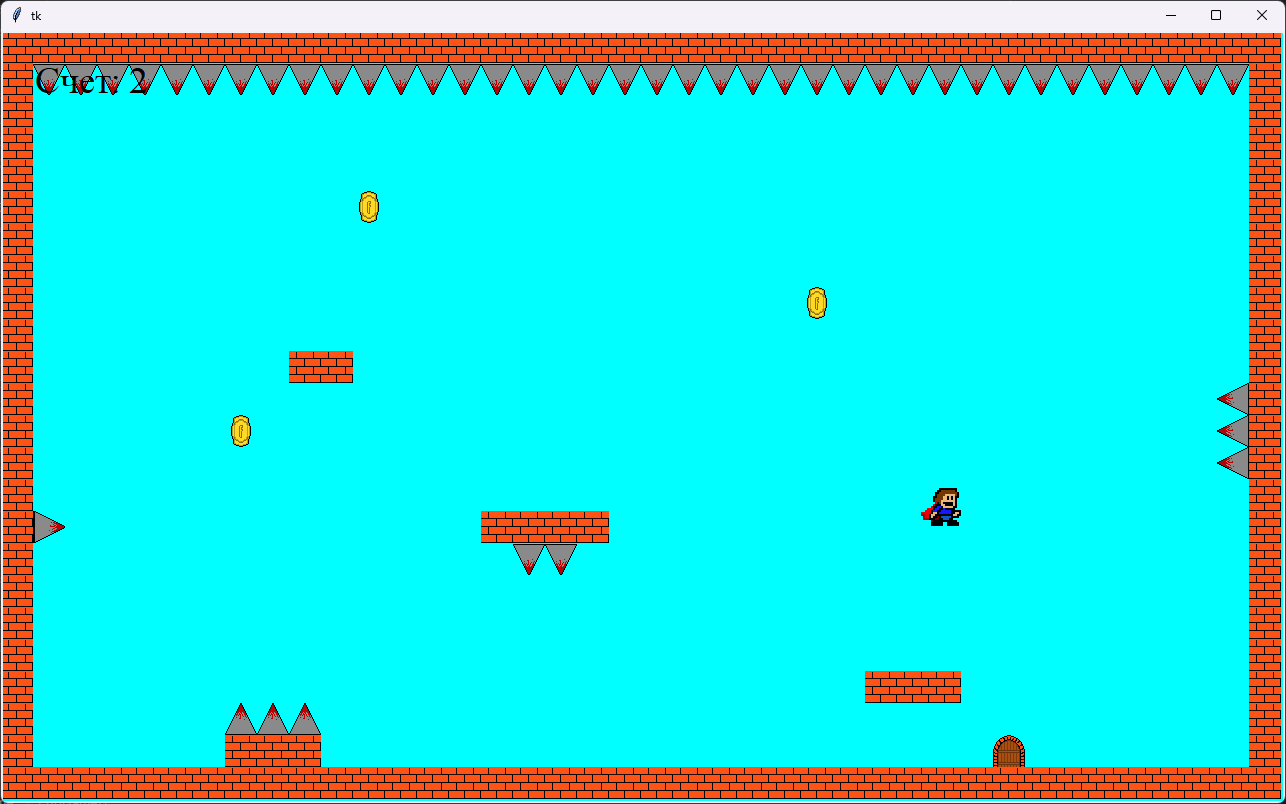
\includegraphics[width=1\linewidth]{menu}}
\caption{Игрок собирает монеты}
\label{menu:image}
\end{figure}

На рисунке \ref{enter:image} игрок собрал все монеты и открыл выход.

\begin{figure}[ht]
\center{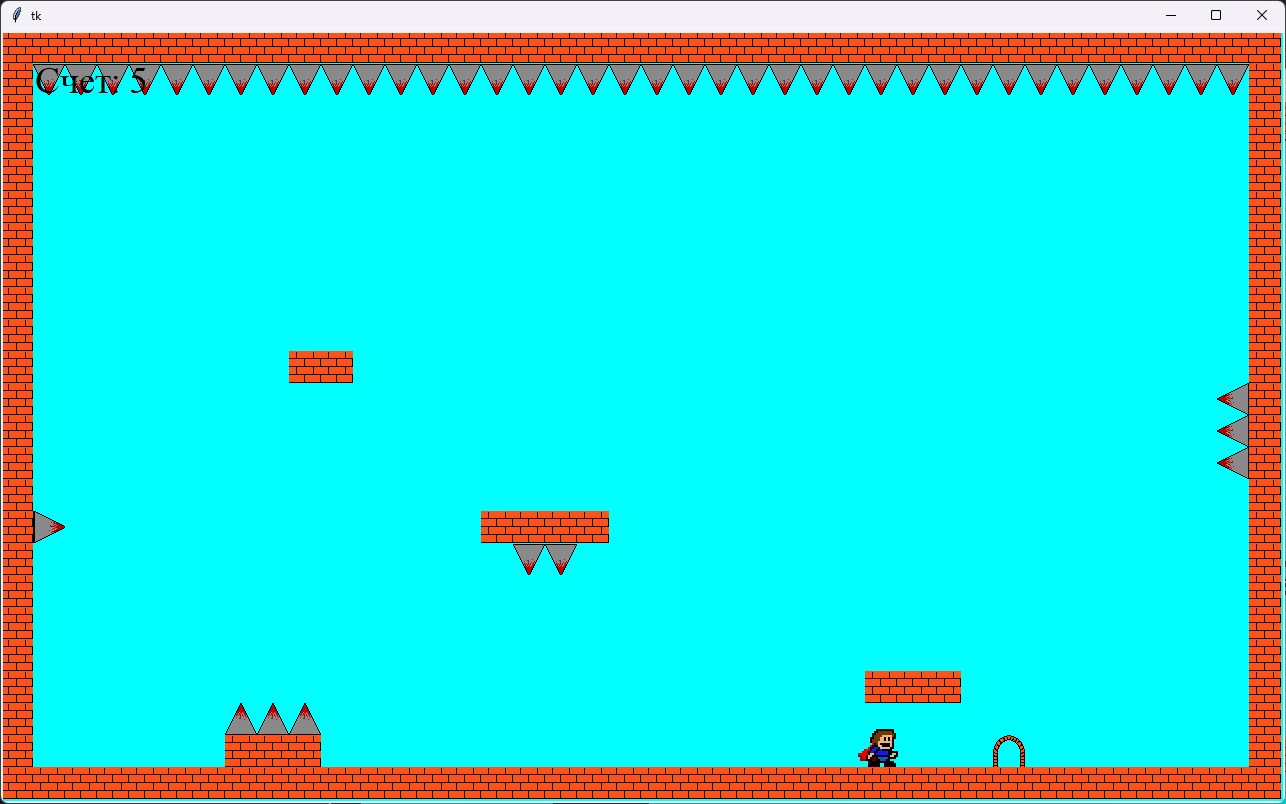
\includegraphics[width=1\linewidth]{enter}}
\caption{Игрок собрал все монеты и открыл выход}
\label{enter:image}
\end{figure}

На рисунке \ref{enter1:image} игрок собрал одну монету и проиграл.

\begin{figure}[ht]
	\center{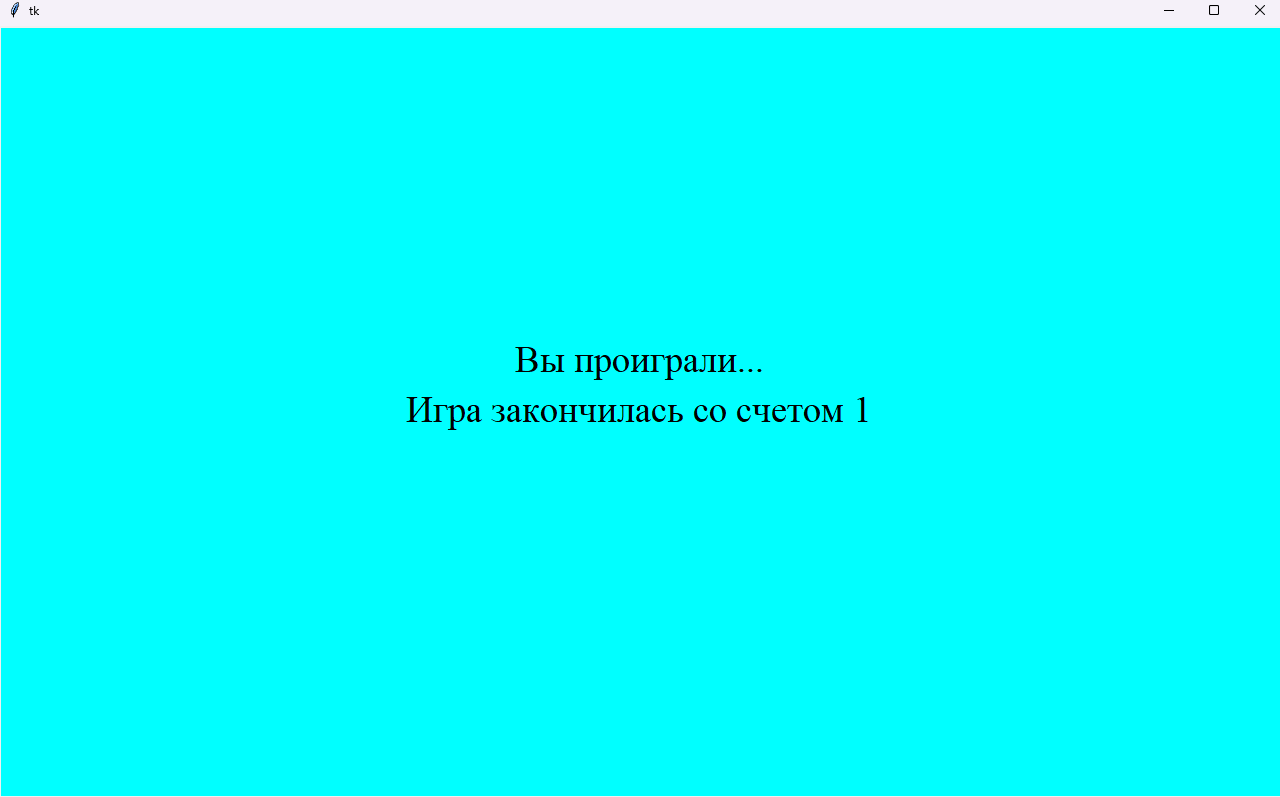
\includegraphics[width=1\linewidth]{enter1}}
	\caption{Игрок собрал одну монету и проиграл}
	\label{enter1:image}
\end{figure}

На рисунке \ref{enter2:image} игрок проиграл не собрав ни одной монеты.

\begin{figure}[ht]
	\center{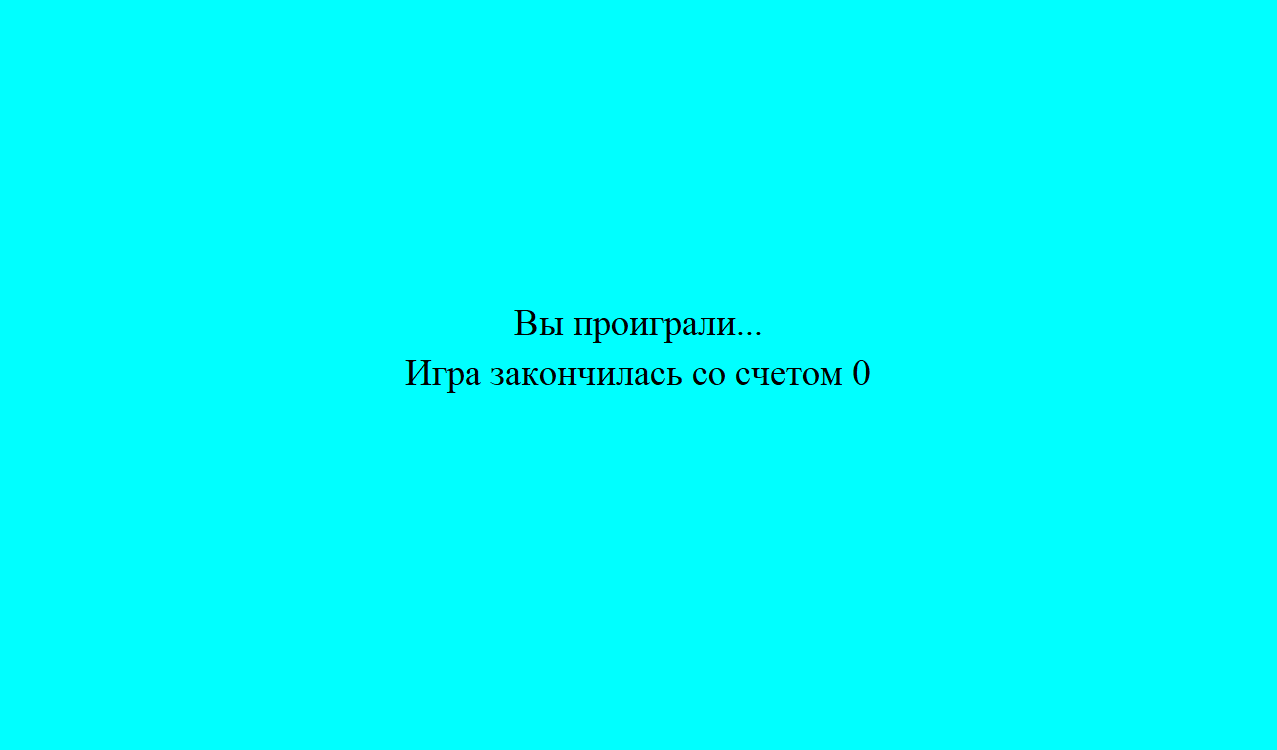
\includegraphics[width=1\linewidth]{enter2}}
	\caption{Игрок проиграл}
	\label{enter2:image}
\end{figure}

На рисунке \ref{enter3:image} игрок собрал все монеты и добрался до выхода.

\begin{figure}[ht]
	\center{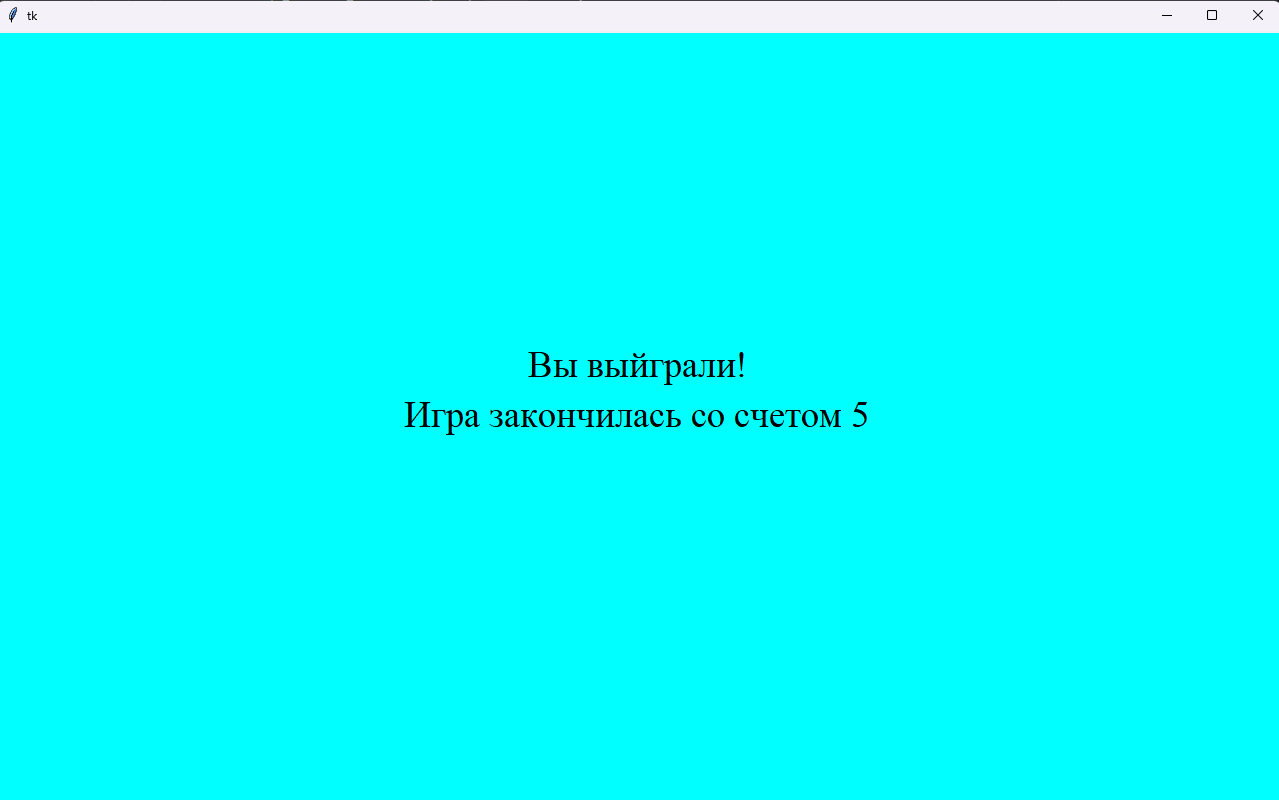
\includegraphics[width=1\linewidth]{enter3}}
	\caption{Игрок собрал все монеты и покинул уровень}
	\label{enter3:image}
\end{figure}